\documentclass[10pt]{beamer}
\usepackage{tikz}
\usepackage{appendixnumberbeamer}
\usepackage{booktabs}
\usepackage[scale=2]{ccicons}
\usepackage{pgfplots}
\usepackage{caption}
\usepackage[backend=biber,style=alphabetic, citestyle=authoryear]{biblatex}

\usetikzlibrary{positioning,automata,arrows,positioning,calc}
\usetheme[progressbar=frametitle]{metropolis}
\usepgfplotslibrary{dateplot}
\setbeamerfont{footnote}{size=\tiny}
\addbibresource{bibliography.bib}

\title{Optimizing Mobility-on-Demand Systems for High Throughput}
\subtitle{Ph.D. Oral Exam}
\author{\textbf{Harshal A. Chaudhari}}
\date{January 16, 2018}

\begin{document}
    % Title frame
    \begin{frame}[plain, noframenumbering]
        \maketitle
        \begin{tikzpicture}[overlay, remember picture]
            \node[above right=.5cm and .8cm of current page.south west]{\includegraphics[scale=0.12]{logos/logo-bu.png}};
        \end{tikzpicture}
    \end{frame}

    % Table of Contents
    % \begin{frame}{Table of Contents}
    %     \setbeamertemplate{section in toc}[sections numbered]
    %     \tableofcontents[hideallsubsections]
    % \end{frame}

    % Problem motivation
    %!TEX root = oral.tex

\section{Problem Motivation}

    \begin{frame}{Mobility-on-Demand Systems}
    \metroset{block=fill}
    \begin{block}{U.S. Department of Transportation}
    ``Mobility-on-Demand (MoD) is an innovative, user-focused approach which leverages emerging mobility services,
    integrated transit networks, real-time data, and cooperative Intelligent Transportation Systems to allow
    for a more traveler-centric transportation, providing improved mobility options to all travelers and users of the system
    in an efficient and safe manner.''
    \end{block}
    \begin{itemize}
        \pause
        \item{\bf Bike-share}: Hubway, NYC CitiBike, etc.
        \pause
        \item{\bf Ride-share}: Zipcar, Car2Go, Enterprise Carshare, etc.
        \pause
        \item{\bf Ride-hail}: Uber, Lyft, etc.
    \end{itemize}
    
    \end{frame}

    \begin{frame}{Common issue of the demand heterogeneity}
        \begin{figure}
            \centering
            {\includegraphics[scale=0.19]{plots/NYC-flow.png}}
            \caption{NYC CitiBike pickups and drop-offs during rush hours\footcite{Liu:2016:RBS:2939672.2939776}.}
        \end{figure}
    \end{frame}

    \begin{frame}{Literature}
    \begin{itemize}
        \item<1->\alert{Modeling:}
            \begin{itemize}
                \item[--]<2-> \textbf{Traffic models:} \textcite{wardrop1900journey,treiber2000congested} \\
            \end{itemize}
        \item<1->\alert{Control:}
            \begin{itemize}
                \item[--]<3-> \textbf{Dynamic Traffic Assignment:} \textcite{friesz1989dynamic,merchant1978optimality,waller2013linear}
                \item[--]<3-> \textbf{Demand analysis:} \textcite{froehlich2008measuring,raviv2013static}, \textcite{schuijbroek2017inventory}
                \item[--]<3-> \textbf{Load balancing:} \textcite{pavone2012robotic}, \textcite{smith2013rebalancing}
            \end{itemize}
        \item<1->\alert{Applications:}
            \begin{itemize}
                \item[--]<4-> \textbf{Taxi dispatch:} \textcite{zhang2017taxi}
                \item[--]<4-> \textbf{Customer incentives:} \textcite{singla2015incentivizing}
                \item[--]<4-> \textbf{Dynamic pricing:} \textcite{castillo2017surge}, \textcite{banerjee2016dynamic}
            \end{itemize}
    \end{itemize}    
    \end{frame}

    %!TEX root = oral.tex

\section{Service Level Requirements}

	\begin{frame}
	\textbf{Paper 1: Inventory Rebalancing and Vehicle Routing in Bike Sharing Systems}
	\begin{itemize}
		\item Jasper Schuijbroek \\
		\textit{Eindhoven University of Technology}
		\item Robert Hampshire \\
		\textit{Carnegie Mellon University}
		\item Willem-Jan van Hoeve \\
		\textit{Carnegie Mellon University}
	\end{itemize}
	\end{frame}

    \begin{frame}{Definition}
    Let $\mathcal{S}$ represent the set of bike sharing stations. For each station $i \in \mathcal{S}$:
    \begin{itemize}
        \item $C_i$ denotes capacity of the station.
        \item Poisson process for bike drop-offs with rate $\lambda_i$
        \item Poisson process for bike pickups  with rate $\mu_i$
    \end{itemize}
    \pause
    The service level requirements at station $i \in \mathcal{S}$ are:
    \begin{eqnarray*}
        \frac{\mathbb{E}[\textrm{Satisfied pickup demands}]}{\mathbb{E}[\textrm{Total pickup demands}]} &\geq& \beta_{i}^{-} \\ \\
        \frac{\mathbb{E}[\textrm{Satisfied dropoff demands}]}{\mathbb{E}[\textrm{Total dropoff demands}]} &\geq& \beta_{i}^{+} \\
    \end{eqnarray*}
    for given $\beta_{i}^{-},\beta_{i}^{+} \in [0,1]$.
    \end{frame}

    \begin{frame}{Markov Chain Formulation}
    Each station is a $M/M/1/K$ queue with $K=C_i$. Markov Chain for inventory $S_i(t)$ is:
    
\begin{center}
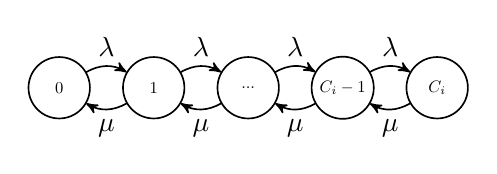
\begin{tikzpicture}[->, >=stealth', auto, semithick, node distance=2cm, state/.style={circle, draw, minimum size=1.3cm, scale=0.6}]
\tikzstyle{every state}=[fill=white,draw=black,thick,text=black,scale=1]
\node[state]    (0)  		{$0$};
\node[state]    (+1)[right of=0]   		{$1$};
\node[state]    (+inf) [right of=+1] 	{$...$};
\node[state]    (+C-1)[right of=+inf]   {$C_i - 1$};
\node[state]	(+C)[right of=+C-1]		{$C_i$};
\path
(0)     edge[bend left]         node{$\lambda$}   (+1)
(+1)    edge[bend left]         node{$\lambda$}   (+inf)
        edge[bend left,below]   node{$\mu$}       (0)
(+inf)  edge[bend left]   		node{$\lambda$}   (+C-1)
		edge[bend left,below]	node{$\mu$}		  (+1)
(+C-1)  edge[bend left]   		node{$\lambda$}   (+C)
		edge[bend left,below]	node{$\mu$}		  (+inf)
(+C)	edge[bend left,below]	node{$\mu$}       (+C-1);	
\end{tikzpicture}
\end{center}
    \begin{itemize}
    	\pause
    	\item[--]$p_i(s, \sigma, t)$ = probability that inventory at station $i$ equals $\sigma$ at time $t \geq 0$ given starting inventory $s$ \\
    	\vspace{0.1in}
    	\pause
    	\item[--]$g_i(s, \sigma) = \frac{1}{T}\int_{0}^{T}p_i(s, \sigma, t) dt$ \\
	\end{itemize}
	\pause
	\textbf{Service Level Requirements:}
    \begin{eqnarray*}
        \frac{\mathbb{E}[\textrm{Satisfied pickup demands}]}{\mathbb{E}[\textrm{Total pickup demands}]} &=& 1 - g_i(s, 0) \\ \\
        \frac{\mathbb{E}[\textrm{Satisfied dropoff demands}]}{\mathbb{E}[\textrm{Total dropoff demands}]} &=& 1 - g_i(s, C_i) \\
    \end{eqnarray*}
    \end{frame}

    \begin{frame}{Service Level Requirements for Hubway}
        \begin{figure}
            \centering
            {\includegraphics[scale=0.17]{plots/hubway_service_level.png}}
            \caption{Observation period 8--9AM on weekdays with $\beta_i^{-}=\beta_i^{+}=95\%$ on Friday, June 1, 2012\footcite{schuijbroek2017inventory}.}
        \end{figure}
        \pause
        \alert{Authors use Maximum Likelihood Estimator for Poisson variables, but they do not have data for unfulfilled demand!}
    \end{frame}

    \section{Routing Problem for bike-share}
    \begin{frame}{Routing Problem}
    \textbf{Problem (P1):} Given $\mathcal{V}$ re-balancing trucks, each with a capacity of $Q$, re-balance the bike inventory such that service level at each station is met, minimize the maximum tour length of the re-balancing truck to obtain $H^*(\mathcal{S}, \mathcal{V})$. \\
    \vspace{0.2in}
    %\baselineskip
    \pause
    \textbf{Constraints:}
    \begin{itemize}
        \item service level
        \item vehicle and station capacity constraints
        \item flow conservation
        \pause
        \item<alert@3>integrality constraints
    \end{itemize}
    \pause
    \alert{Pure MIP approach: Intractable for realistic scenarios with $|\mathcal{S}| \geq 50$ and $|\mathcal{V}| \geq 3$.}
    \end{frame}

    \section{Clustered Routing Problem}
    \begin{frame}{Clustered Routing Problem}
    \textbf{Problem (P2):} Find a clustering solution that assigns disjoint clusters of stations $\mathcal{S}_v \subseteq \mathcal{S}$ to vehicles
    $v \in \mathcal{V}$ such that the service level requirements can be satisfied using \textit{only} within-cluster vehicle routing. \\
    \pause
    \begin{itemize}
        \item Extended set-partitioning problem.
        \pause
        \item Approximate within-cluster routing costs.
        \pause
        \item<alert@4>{Impose triangle inequality -- within-cluster routing costs lower bounded by length of shortest Hamiltonian path.}
    \end{itemize}
    \pause
    \textbf{Maximum Spanning Star approximation:} \pause $SPS_i(\mathcal{S}_v) = \sum_{j \in \mathcal{S}_v}d_{ij}$.
    \pause
    Maximum-cost spanning star \bigg($\max_{i \in \mathcal{S}_v}SPS_i(\mathcal{S}_v)$\bigg) approximates within-cluster routing cost.
    \end{frame}

    \begin{frame}{Heuristic 1}
    \textbf{Clustered MIP (H1):} \only<2->{\alert{(Sub-optimal)}}
    \begin{enumerate}
        \item Solve (P2)
        \item Solve (P1) for each cluster of stations $\mathcal{S} = \mathcal{S}_v$ and $\mathcal{V} = \{v\}$ to obtain $H^*(\mathcal{S}_v, \{v\})$
        \item $H^* = \max_{v \in \mathcal{V}}H^*(\mathcal{S}_v, \{v\})$
    \end{enumerate}
    \end{frame}
    \begin{frame}{Heuristic 2}
    \textbf{Clustered MIP with Cuts (H2):}
    \begin{enumerate}
        \item Initialize a cut set of stations $\mathcal{C} = \emptyset$
        \item Solve (P2) with additional constraint $\forall v: \mathcal{S}_v \not \subseteq \mathcal{C}$ to obtain $H^*$
        \item Solve (P1) for each cluster of stations $\mathcal{S} = \mathcal{S}_v$ and $\mathcal{V} = \{v\}$ to obtain $H^*(\mathcal{S}_v, \{v\})$
            \begin{itemize}
                \item If $\max_{v \in \mathcal{V}}H^*(\mathcal{S}_v, \{v\}) < H^*$ or $\mathcal{C}=\emptyset$, redefine $H^*$ and store routing solution.
                \item For each $v \in \mathcal{V}$ with $H^*(\mathcal{S}_v, \{v\}) \geq H^*$, redefine $\mathcal{C} = \mathcal{C} \cup \{\mathcal{S}_v\}$ 
            \end{itemize}
        \item Go to step 2.
    \end{enumerate}
    \pause
    \alert{Break sub-optimal clusters by dividing their stations over many different vehicles.}
    \end{frame}

    \begin{frame}{Computation Results for Hubway}
        \begin{figure}
            \centering
            {\includegraphics[scale=0.28]{plots/clustered_MIP.png}}
            \caption{Averaged results over 41 runs of algorithms\footcite{schuijbroek2017inventory}.}
        \end{figure}
    \end{frame}

    \begin{frame}{Summary}
    	\textbf{Positives:}
    	\begin{itemize}
    		\item Simple framework for evaluating service level requirements.
    		\item Heuristic algorithm for re-balancing problem in bike-share.
    	\end{itemize}
    		\vspace{0.1in}
    		\pause
    	\textbf{Concerns:}
    	\begin{itemize}
    		\item \alert{Tradeoff between routing costs and revenue loss due to imbalance.}
    		\item \alert{Assumption of negligible demand during the re-balancing operation.}
    	\end{itemize}
    \end{frame}

    %!TEX root = oral.tex

\section{Routing problem for autonomous ride-share}

	\begin{frame}
	\textbf{Paper 2: Robotic load balancing for mobility-on-demand systems}
	\begin{itemize}
		\item Marco Pavone \\
		\textit{Stanford University}
		\item Stephen L. Smith \\
		\textit{University of Waterloo}
		\item Emilio Frazzoli \\
		\textit{Massachusetts Institute of Technology}
		\item Daniela Rus \\
		\textit{Massachusetts Institute of Technology}
	\end{itemize}
	\end{frame}

    \begin{frame}{Fluid model}
        \begin{figure}
            \centering
            {\includegraphics[scale=0.28]{plots/fluid_model.png}}
            \caption{Fluid model for autonomous cars\footcite{pavone2012robotic}.}
        \end{figure}
    \end{frame}

    \begin{frame}{Existence of equilibrium}
    Let $\mathcal{A}$ be set of assignments of $\alpha$ that verify equation
    \begin{equation*}
    \sum_{j \neq i}\alpha_{ij} + \lambda_i = \sum_{j \neq i}\alpha_{ji} + \sum_{j \neq i}\lambda_j p_{ji}
    \end{equation*}
    for each $i \in \mathcal{S}$, 
    \pause
    and let
    \begin{equation*}
    V_{\alpha} = \sum_{ij} T_{ij}(p_{ij} \lambda_i + \alpha_{ij})
    \end{equation*}
    \pause
    then,
    \begin{enumerate}
        \item if $V > V_\alpha$, then there exists an equilibrium assignment of $\alpha$.
        \item if $V \leq V_\alpha$, then no equilibrium exists.
    \end{enumerate}
    \pause
    \alert{$V^* = \min_{\alpha \in \mathcal{A}}V_{\alpha}$ is minimum number of vehicles required for existence of equilibrium.}
    \end{frame}

    \begin{frame}{Optimal Re-balancing}
    Minimize
    \begin{equation*}
    \sum_{ij} T_{ij}\alpha_{ij}
    \end{equation*}
    subject to
    \begin{align*}
        \sum_{j \neq i}\alpha_{ij} + \lambda_i = \sum_{j \neq i}\alpha_{ji} + \sum_{j \neq i}\lambda_j p_{ji} && \forall i \in \mathcal{S} \\
        \alpha_{ij} \geq 0 && \forall{i,j} \in \mathcal{S}
    \end{align*}
    \pause
    \only<2>{\alert{Minimizing $\sum_{ij} T_{ij}\alpha_{ij}$ also leads to minimizing $V_\alpha$ (total vehicle utilization).}}
    \pause
    If we impose triangle inequality on travel times $T_{ij}$, then stations can be divided into those with a \textit{surplus} ($S$) and those with a \textit{deficit} ($D$), where $S = \big\{i \in \mathcal{S} | \lambda_i < \sum_j \lambda_j p_{ji}\big\}$ and $D = \mathcal{S} \setminus S$.
    \end{frame}

    \begin{frame}{Continuous bipartite matching}
    Minimize
    \begin{equation*}
    \sum_{i \in S, j \in D} T_{ij}\alpha_{ij}
    \end{equation*}
    subject to
    \begin{align*}
        \sum_{j \in D}\alpha_{ij} = - \lambda_i + \sum_{j \neq i}\lambda_j p_{ji} && \forall i \in S \\
        \sum_{i \in S}\alpha_{ij} = \lambda_j - \sum_{i \neq j}\lambda_i p_{ij} && \forall j \in D \\
        \alpha_{ij} \geq 0 && \forall{i,j} \in \mathcal{S}
    \end{align*}
    \pause
    \begin{itemize}
        \item Fewer variables and fewer constraints.
        \pause
        \item Linear Program.
    \end{itemize}
    \end{frame}

    \begin{frame}{Summary}
    	\textbf{Positives:}
    	\begin{itemize}
    		\item Fluid models make it easy to analyze system dynamics.
    		\item Allows us to study stability of equilibrium.
    	\end{itemize}
    		\vspace{0.1in}
    		\pause
    	\textbf{Concerns:}
    	\begin{itemize}
    		\item \alert{Only for the case of constant flow rates.}
    		\item \alert{Susceptible to perturbations in $p_{ij}$.}
    	\end{itemize}
    \end{frame}

    %!TEX root = oral.tex

\section{Role of dynamic pricing in Uber}

	\begin{frame}
	\textbf{Paper 3: Surge Pricing Solves the Wild Goose Chase}
	\begin{itemize}
		\item Juan Camilo Castillo \\
		\textit{Stanford University}
		\item Dan Knoepfle \\
		\textit{Uber Technologies}
		\item E. Glen Weyl \\
		\textit{Microsoft Research}
	\end{itemize}
	\end{frame}

    \begin{frame}{Ride Hailing}
    \begin{itemize}
        \item Uber, Lyft: more efficient matching technology than taxis
        \begin{itemize}
            \item \textcite{cramer2016disruptive}: Utilization rate increases by 30--50\%
            \item Potential welfare gain is substantial \\
        \end{itemize}
        \pause
        \item Challenges to get market design right
        \begin{itemize}
            \item Matching passengers with drivers
            \item Pricing (dynamic?)
        \end{itemize}
    \end{itemize}
    % \pause
    % \alert{Surge Pricing solves a matching failure!}
    \end{frame}

    \begin{frame}{Wild Goose Chases (WGCs)}
    Ride-hailing systems are prone to \textit{wild goose chases}
    \pause
    \begin{itemize}
        \item Too many ride requests
        \item Drivers spend more time picking up passengers
        \item Number of completed trips drop
    \end{itemize}
    \pause
    \metroset{block=fill}
    \only<3>{
    \begin{block}{Driver Life:}
    	\centering
    	\large{Idle Time} $\rightarrow$ \large{Pickup Time} $\rightarrow$ \large{Travel Time}
    \end{block}
    }
    \pause
    \only<4->{
    \begin{block}{Driver Life:}
    	\centering
    	\large{Idle Time} $\rightarrow$ \alert{\large{Pickup Time}} $\rightarrow$ \large{Travel Time}
    \end{block}
    }
    % \pause
    % \only<3>{\alert{Street-hail cabs do not face the same problem!}}
    \pause
    Research problem: How to avoid Wild Goose Chases?
    \pause
    \begin{itemize}
        \item WGCs can be avoided by setting higher prices
        %\item With uniform pricing: higher costs \textit{always}
        %\item With dynamic pricing: lower costs during low demand
    \end{itemize}
    \end{frame}

    \begin{frame}{Notations}
    	\begin{itemize}
    		\item $T$ : Waiting time for customer = Pickup time for driver
    		\pause
    		\item $p$ : Price point
    		\pause
    		\item $L$ : Labor supply (total number of drivers)
    		\pause
    		\item $Q$ : Quantity (total number of completed rides)
    		\pause
    		\item $D(T, p)$ : Demand function
    		\pause
    		\item $S(T, L)$ : Supply function
    	\end{itemize}
    \end{frame}

    \begin{frame}{Demand}
        \begin{figure}
            \centering
            {\includegraphics[scale=0.30]{plots/demand.png}}
            \caption{Demand curve\footcite{castillo2017surge}.}
        \end{figure}
    \end{frame}

    \begin{frame}{Supply}
        \begin{figure}
            \centering
            {\includegraphics[scale=0.30]{plots/supply.png}}
            \caption{Supply curve\footcite{castillo2017surge}.}
        \end{figure}
    \end{frame}

    \begin{frame}{Empirical supply}
        \begin{figure}
            \centering
            {\includegraphics[scale=0.35]{plots/empirical_supply.png}}
            \caption{Quintiles of empirical supply\footcite{castillo2017surge}.}
        \end{figure}
    \end{frame}

    \begin{frame}{Equilibrium}
        \begin{figure}
            \centering
            {\includegraphics[scale=0.30]{plots/equilibrium.png}}
            \caption{Equilibrium point\footcite{castillo2017surge}.}
        \end{figure}
    \end{frame}

    \begin{frame}{Equilibrium}
        \begin{figure}
            \centering
            {\includegraphics[scale=0.30]{plots/equilibrium_0.png}}
            \caption{Equilibrium point.}
        \end{figure}
    \end{frame}

    % \begin{frame}{Wild Goose Chase}
    %     \begin{figure}
    %         \centering
    %         {\includegraphics[scale=0.30]{plots/wild_goose_chase.png}}
    %         \caption{Wild Goose Chase\footcite{castillo2017surge}.}
    %     \end{figure}
    % \end{frame}

    \begin{frame}{Wild Goose Chase}
        \begin{figure}
            \centering
            {\includegraphics[scale=0.30]{plots/wild_goose_chase_0.png}}
            \caption{Wild Goose Chase.}
        \end{figure}
    \end{frame}

    \begin{frame}{Wild Goose Chase}
        \begin{figure}
            \centering
            {\includegraphics[scale=0.30]{plots/wild_goose_chase_1.png}}
            \caption{Wild Goose Chase.}
        \end{figure}
    \end{frame}

    % \begin{frame}{Market Collapse}
    %     \begin{figure}
    %         \centering
    %         {\includegraphics[scale=0.30]{plots/market_collapse.png}}
    %         \caption{Market Collapse\footcite{castillo2017surge}.}
    %     \end{figure}
    % \end{frame}

    \begin{frame}{Market Collapse}
        \begin{figure}
            \centering
            {\includegraphics[scale=0.30]{plots/market_collapse_0.png}}
            \caption{Market Collapse.}
        \end{figure}
    \end{frame}

    \begin{frame}{Market Collapse}
        \begin{figure}
            \centering
            {\includegraphics[scale=0.30]{plots/market_collapse_1.png}}
            \caption{Market Collapse.}
        \end{figure}
    \end{frame}

    \begin{frame}{Pricing for Strong vs. Weak Market}
    	\large{Welfare = Customer Utility + Driver earnings + Platform earnings} \\
    	\pause
    	\textbf{Weak market} = low demand (11am-noon) \\
    	\textbf{Strong market} = high demand (6pm-7pm)
    	\pause
    	\only<3>{
        \begin{figure}
            \centering
            {\includegraphics[scale=0.35]{plots/weak_strong_market_0.png}}
            \caption{Need for dynamic pricing\footcite{castillo2017surge}.}
        \end{figure}
        }
        \pause
        \only<4>{
        \begin{figure}
            \centering
            {\includegraphics[scale=0.35]{plots/weak_strong_market_1.png}}
            \caption{Need for dynamic pricing\footcite{castillo2017surge}.}
        \end{figure}
        }
    \end{frame}

    \begin{frame}{Summary}
    	\textbf{Positives:}
    	\begin{itemize}
    		\item Formulation of endogenous relationship between supply and demand.
    	\end{itemize}
    		\vspace{0.1in}
    		\pause
    	\textbf{Concerns:}
    	\begin{itemize}
    		\item \alert{Location-based discrimination?}
    		\item \alert{Oblivious to re-balancing problem. Uber POV - surge pricing helps with re-balancing.}
    	\end{itemize}
    \end{frame}

    %!TEX root = oral.tex

\section{Open Problems}

	\begin{frame}{Discussion}
		\begin{itemize}
			\item \textbf{Strategic drivers} \\
			Putting Data in the Driver's Seat: Optimizing Earnings for On-Demand Ride-Hailing
			\textit{\small (To appear in WSDM 2018 proceedings)}
			\pause
			\item \textbf{Effect of strategic drivers on the platform}
			\textit{(Work in progress)}
			\pause
			\item \textbf{Robust Re-balancing strategies}
			\pause
			\item \textbf{Maintaining service levels with strategic market design}
			\pause
			\item \textbf{Optimal earning strategies for human drivers in presence of autonomous agents}
			\pause
			\item \textbf{Strategic platform monitoring} \\
			Efficient Markov Chain Monitoring
			\textit{\small (To appear in SDM 2018 proceedings)}
		\end{itemize}
	\end{frame}

	% Thank You slide
    \begin{frame}
        \centering
        \Huge{\textsc{Thank You!}}
    \end{frame}

    % Bibliography
    \begin{frame}[allowframebreaks]{References}
        \printbibliography
    \end{frame}

\end{document}
